\documentclass[a4paper, 14pt]{extarticle}

\usepackage{../generalPreamble}
\usepackage{../reportFormat}
\setcounter{MaxMatrixCols}{20}

\newcommand\sbullet[1][.5]{\mathbin{\vcenter{\hbox{\scalebox{#1}{$\bullet$}}}}}

\begin{document}

\begin{titlepage}
    \centering
    {\bfseries
        \uppercase{
            Минобрнауки России \\
            Санкт-Петербургский государственный \\
            Электротехнический университет \\
            \enquote{ЛЭТИ} им. В.И.Ульянова (Ленина)\\
        }
        Кафедра ИБ

        \vspace{\fill}
        \uppercase{Лабораторная работа №4} \\
        по дисциплине \enquote{Криптография и защита информации} \\
        Тема: Изучение шифра DES
    }

    \vspace{\fill}
    \begin{tabularx}{0.8\textwidth}{l X c r}
        Студент гр. 6304 & & \underline{\hspace{3cm}} & Корытов П.В.\\
        Преподаватель & & \underline{\hspace{3cm}} & Племянников А.К.
    \end{tabularx}

    \vspace{1cm}
    Санкт-Петербург \\
    \the\year{}
\end{titlepage}

\newpage

\section*{Цель работы}
Цель работы: исследовать шифры Hill, ADFGVX, Playfair и получить практические навыки работы с ними, в том числе и в программном продукте CrypTool 1 и 2.

\section{Исследование преобразований DES}
\subsection{Описание}%
\label{sub:des_descr}
DES (англ. Data Encryption Standart) --- стандарт шифрования данных --- блочный шифр с симетричными ключами. Разработан NIST (National Institute of Standarts and Technology).

\subsubsection{Сеть Фейстеля}
Шифр DES основан на сети Фейстеля (см. рисунок~\ref{img:1:1}). Принцип работы сети следующий:

\begin{figure}[h]
    \centering
    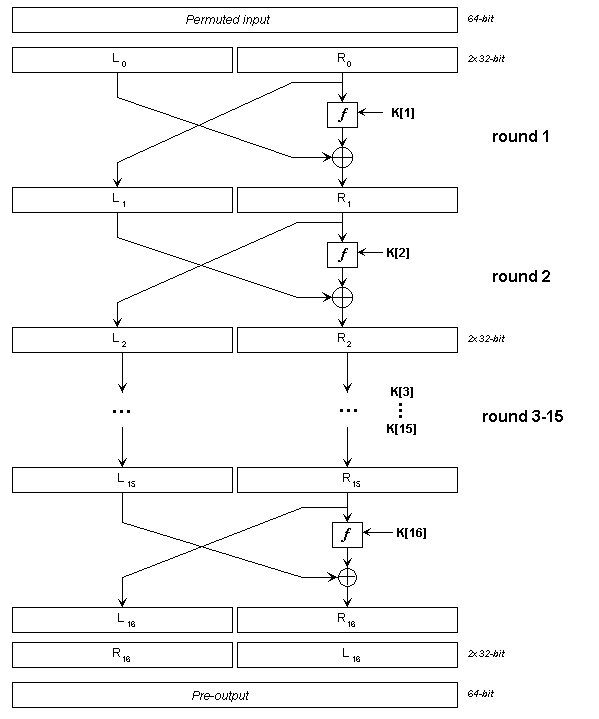
\includegraphics[width=0.7\textwidth]{./img/S001.jpg}
    \caption{Сеть Фейстеля}%
    \label{img:1:1}
\end{figure}

\begin{enumerate}
    \item Выбранный блок делится на два равных субблока $L_0$ и $R_0$
    \item $R_0$ преобразуется функцией шифра $f(R_0, K_0)$, после чего складывается по модулю 2 с $L_0$
    \item Результат сложения становится $R_1$, а $R_0$ становится $L_1$ для следующего раунда
    \item Операция повторяется $N-1$ раз. При переходе между раундами меняются раундовые ключи $K_0, K_1, \ldots $.\\
\end{enumerate}
Т.е.:
\[ L_i = R_{i-1}; \]
\[ R_i = L_{i-1} \oplus f(R_{i-1}), \]
где $i$ --- номер текущего рауда, $K_i$ --- ключ раунда.

В шифре DES размер блока --- 64 бита, число раундов --- 16. Перед входом в сеть производится начальная перестановка.

\FloatBarrier{}

\subsubsection{Структура раудовой функции}
Структура функции представлена на рисунке~\ref{img:1:2}.
\begin{figure}[h]
    \centering
    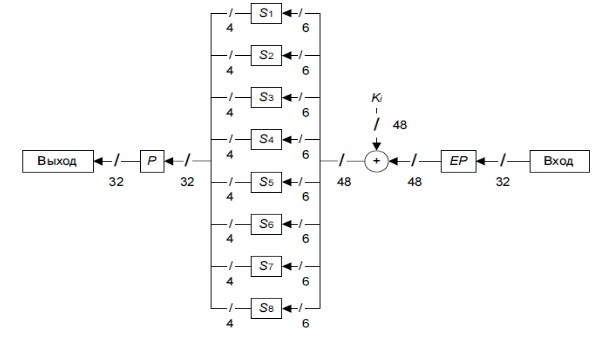
\includegraphics[width=0.9\textwidth]{./img/S002.jpg}
    \caption{Структура $f$}%
    \label{img:1:2}
\end{figure}

Этапы функции:
\begin{enumerate}
    \item Расширяющая перестановка, преобразует 32 бита в 48 бит (рисунок~\ref{img:1:3})
        \begin{figure}[h]
            \centering
            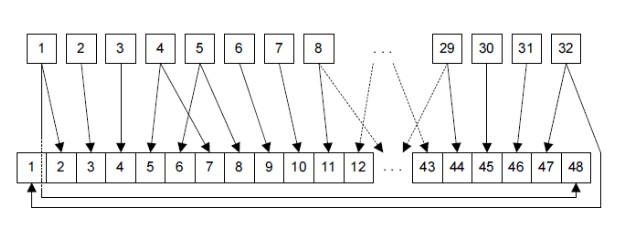
\includegraphics[width=0.9\textwidth]{./img/S003.jpg}
            \caption{Расширящая перестановка}%
            \label{img:1:3}
        \end{figure}
    \item Полученные 48 бит складываются с $K_i$ операцией xor (рисунок~\ref{img:1:3_1})
        \begin{figure}[h]
            \centering
            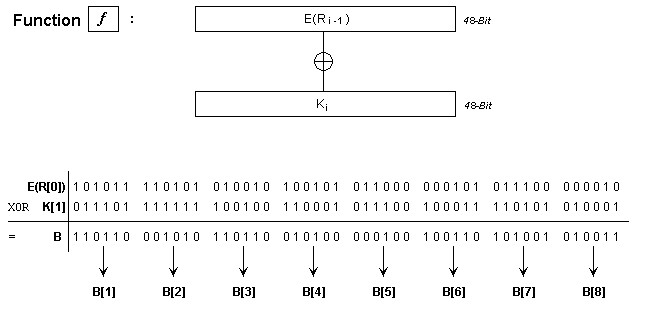
\includegraphics[width=0.8\textwidth]{./img/S007.jpg}
            \caption{Побитовое сложение}%
            \label{img:1:3_1}
        \end{figure}
        
    \item Результат сложения разбивается на 8 блоков по 6 битов. Каждый блок обрабатывается соответствующей таблицей замен (рис.~\ref{img:1:3_2}).
    \begin{itemize}
        \item Первый и последний биты составляют стороку
        \item Средние 4 бита --- номер столбца\\
    \end{itemize}
    \begin{figure}[h]
        \centering
        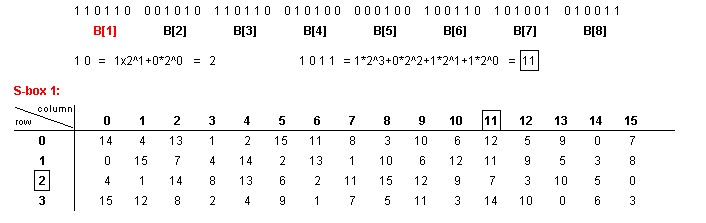
\includegraphics[width=\textwidth]{./img/S008.jpg}
        \caption{Таблица замен}%
        \label{img:1:3_2}
    \end{figure}

    Таблицы замен для каждого блока свои.

    \item Над полученными 32 битами, после выполнения замен, выполняется перестановка ($P$)
\end{enumerate}

\subsubsection{Генерация раундовых ключей}
Генерация раундовых ключей представлена на рисунке~\ref{img:1:4}.
\begin{figure}[h]
    \centering
    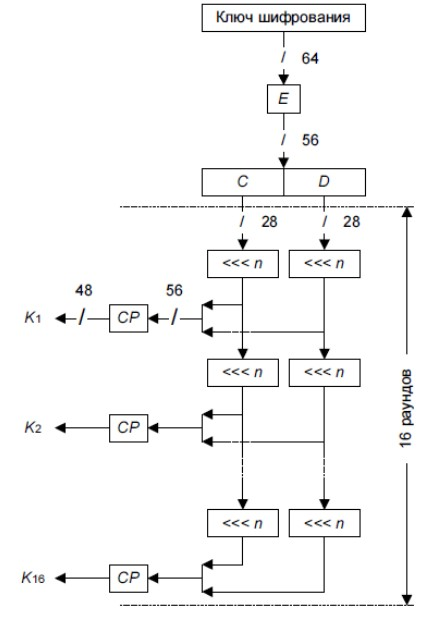
\includegraphics[width=0.5\textwidth]{./img/S004.jpg}
    \caption{Генерация раундовых ключей}%
    \label{img:1:4}
\end{figure}
Из 64-битного ключа используется только 56 бит --- каждый 8-й бит исключается. После выполняется перестановка ($E$).

После перестановки блок в 56 бит делится на два 28-битных блока ($C$, $D$). Затем выполняются 16 раудов преобразований:
\begin{enumerate}
    \item Текущие $C, D$ циклически сдвигаются влева на определенное количество бит
    \item $C, D$ объединяются в 56-битное значение, к которому применяется сжимающая перестановка $CP$. Получается 48-битный ключ.
\end{enumerate}


\FloatBarrier{}
\subsection{Формулировка задания}

\begin{enumerate}
    \item Изучить преобразования шифра DES с помощью демонстрационного приложения из Cryptool 1.
        \begin{itemize}
            \item Indiv.Procedures-> Visualization…-> DES…
        \end{itemize}
    \item Выполнить вручную преобразования одного раунда и вычисление раундовых ключей при следующих исходных данных:
        \begin{itemize}
            \item Открытый текст (не более 64 бит) – фамилия\_имя (транслитерация латиницей)
            \item Ключ (56 бит) – номер зачетной книжки II инициал (всего 7 символов)
        \end{itemize}
    \item Выполнить вручную обратное преобразование зашифрованного сообщения
\end{enumerate}

\subsection{Ход работы}
\begin{enumerate}
    \item С помощью демонстрационного приложения изучена работа шифра. В~\ref{sub:des_descr} вставлены скриншоты.
    \item Проведено ручное преобразование одного раунда.\\
    Открытый текст --- \texttt{KORYTOVP}, ключ --- \texttt{0630417}. Перестановки выбраны отсутствующие.
    \item Произведено преобразование в бинарный формат:
    \begin{itemize}
        \item \texttt{KORYTOVP} --- \texttt{01001011 01001111 01010010 01011001 01010100 01001111 01010110 01010000}
        \item \texttt{0630417} --- \texttt{00110000 00110110 00110011 00110000 00110100 00110001 00110111}\\
    \end{itemize}
    В матричном виде:
    \begin{equation}%
        \label{eq:input}
        I = \begin{bmatrix}
            0   & 0   & 0   & 0   & 0   & 0   & 0   & 0   \\
            1   & 1   & 1   & 1   & 1   & 1   & 1   & 1   \\
            0   & 0   & 0   & 0   & 0   & 0   & 0   & 0   \\
            0   & 0   & 1   & 1   & 1   & 0   & 1   & 1   \\
            1   & 1   & 0   & 1   & 0   & 1   & 0   & 0   \\
            0   & 1   & 0   & 0   & 1   & 1   & 1   & 0   \\
            1   & 1   & 1   & 0   & 0   & 1   & 1   & 0   \\
            1   & 1   & 0   & 1   & 0   & 1   & 0   & 0   \\
        \end{bmatrix}; K = \begin{bmatrix}
            0   & 0   & 0   & 0   & 0   & 0   & 0   \\
            0   & 0   & 0   & 0   & 0   & 0   & 0   \\
            1   & 1   & 1   & 1   & 1   & 1   & 1   \\
            1   & 1   & 1   & 1   & 1   & 1   & 1   \\
            0   & 0   & 0   & 0   & 0   & 0   & 0   \\
            0   & 1   & 0   & 0   & 1   & 0   & 1   \\
            0   & 1   & 1   & 0   & 0   & 0   & 1   \\
            0   & 0   & 1   & 0   & 0   & 1   & 1   \\
        \end{bmatrix}
    \end{equation}
    \item Сначала нужно вычислить раундовый ключ. Из таблиц DES взята перестановка PC1:
    \begin{equation}
        PC1 = \begin{bmatrix}
            57  & 49  & 41  & 33  & 25  & 17  & 9   \\
            1   & 58  & 50  & 42  & 34  & 26  & 18  \\
            10  & 2   & 59  & 51  & 43  & 35  & 27  \\
            19  & 11  & 3   & 60  & 52  & 44  & 36  \\
            63  & 55  & 47  & 39  & 31  & 23  & 15  \\
            7   & 62  & 54  & 46  & 38  & 30  & 22  \\
            14  & 6   & 61  & 53  & 45  & 37  & 29  \\
            21  & 13  & 5   & 28  & 20  & 12  & 4   \\
        \end{bmatrix}
    \end{equation}
    К ключу добавлен ещё один пустой столбец, произведена перестановка:

    \begin{equation}
        K_{perm} = PC1(K) = \begin{bmatrix}
            0   & 0   & 0   & 0   & 1   & 1   & 0   \\
            0   & 0   & 1   & 1   & 0   & 1   & 1   \\
            0   & 0   & 1   & 1   & 0   & 0   & 1   \\
            1   & 0   & 0   & 0   & 0   & 0   & 0   \\
            1   & 1   & 1   & 0   & 1   & 1   & 0   \\
            0   & 1   & 0   & 0   & 0   & 1   & 1   \\
            0   & 0   & 0   & 0   & 1   & 0   & 1   \\
            1   & 0   & 0   & 1   & 1   & 0   & 0   \\
        \end{bmatrix}
    \end{equation}

    \item Ключ разделен на две части, произведен циклический сдвиг:
    \begin{equation}
        \begin{array}{c}
            K_L = \begin{bmatrix}
                0   & 0   & 0   & 0   & 1   & 1   & 0   \\
                0   & 0   & 1   & 1   & 0   & 1   & 1   \\
                0   & 0   & 1   & 1   & 0   & 0   & 1   \\
                1   & 0   & 0   & 0   & 0   & 0   & 0   \\
            \end{bmatrix}\\
            \\
            K_R = \begin{bmatrix}
                0   & 1   & 1   & 1   & 0   & 1   & 1   \\
                1   & 0   & 1   & 0   & 0   & 0   & 1   \\
                1   & 0   & 0   & 0   & 0   & 1   & 0   \\
                0   & 1   & 0   & 0   & 1   & 1   & 0   \\
            \end{bmatrix}
        \end{array} \Rightarrow{} K_{roll1} = 
        \begin{bmatrix}
            >> K_L\\
            >> K_R
        \end{bmatrix} =
        \begin{bmatrix}
            0   & 0   & 0   & 0   & 0   & 1   & 1   \\
            1   & 0   & 0   & 1   & 1   & 0   & 1   \\
            1   & 0   & 0   & 1   & 1   & 0   & 0   \\
            0   & 1   & 0   & 0   & 0   & 0   & 0   \\
            0   & 1   & 1   & 1   & 0   & 1   & 1   \\
            1   & 0   & 1   & 0   & 0   & 0   & 1   \\
            1   & 0   & 0   & 0   & 0   & 1   & 0   \\
            0   & 1   & 0   & 0   & 1   & 1   & 0   \\
        \end{bmatrix}
    \end{equation}
    \item К сдвинутому ключу применена перестановка PC2. Получен первый раундовый ключ
    \begin{equation}\label{eq:k1}
        PC2 = \begin{bmatrix}
            14  & 17  & 11  & 24  & 1   & 5   \\
            3   & 28  & 15  & 6   & 21  & 10  \\
            23  & 19  & 12  & 4   & 26  & 8   \\
            16  & 7   & 27  & 20  & 13  & 2   \\
            41  & 52  & 31  & 37  & 47  & 55  \\
            30  & 40  & 51  & 45  & 33  & 48  \\
            44  & 49  & 39  & 56  & 34  & 53  \\
            46  & 42  & 50  & 36  & 29  & 32  \\
        \end{bmatrix}; K_1 = PC2(K_{roll1}) = \begin{bmatrix}
            1   & 0   & 1   & 0   & 0   & 0   \\
            0   & 0   & 1   & 1   & 0   & 0   \\
            1   & 1   & 1   & 0   & 0   & 1   \\
            0   & 1   & 0   & 0   & 0   & 0   \\
            0   & 0   & 1   & 0   & 0   & 1   \\
            1   & 0   & 1   & 0   & 0   & 1   \\
            0   & 0   & 0   & 0   & 1   & 0   \\
            0   & 1   & 0   & 1   & 0   & 1   \\
        \end{bmatrix}
    \end{equation}
    \item Ко входному тексту (\ref{eq:input}) применена перестановка IP:\@
    \begin{equation}\label{eq:ip}
        \begin{bmatrix}
            58  & 50  & 42  & 34  & 26  & 18  & 10  & 2   \\
            60  & 52  & 44  & 36  & 28  & 20  & 12  & 4   \\
            62  & 54  & 46  & 38  & 30  & 22  & 14  & 6   \\
            64  & 56  & 48  & 40  & 32  & 24  & 16  & 8   \\
            57  & 49  & 41  & 33  & 25  & 17  & 9   & 1   \\
            59  & 51  & 43  & 35  & 27  & 19  & 11  & 3   \\
            61  & 53  & 45  & 37  & 29  & 21  & 13  & 5   \\
            63  & 55  & 47  & 39  & 31  & 23  & 15  & 7   \\
        \end{bmatrix}
    \end{equation}
    \begin{equation}
        I_{perm} = IP(I) = \begin{bmatrix}
            1   & 1   & 1   & 1   & 0   & 0   & 1   & 0   \\
            1   & 0   & 0   & 1   & 1   & 0   & 1   & 0   \\
            1   & 1   & 1   & 1   & 0   & 0   & 1   & 0   \\
            0   & 0   & 0   & 0   & 1   & 0   & 1   & 0   \\
            1   & 1   & 0   & 1   & 0   & 0   & 1   & 0   \\
            0   & 1   & 0   & 0   & 1   & 0   & 1   & 0   \\
            0   & 0   & 1   & 0   & 1   & 0   & 1   & 0   \\
            0   & 1   & 1   & 0   & 1   & 0   & 1   & 0   \\
        \end{bmatrix}
    \end{equation}
    \item Текст разделен на два блока:
    \begin{equation}
        \begin{array}{c}
            L_0 = \begin{bmatrix}
                1   & 1   & 1   & 1   & 0   & 0   & 1   & 0   \\
                1   & 0   & 0   & 1   & 1   & 0   & 1   & 0   \\
                1   & 1   & 1   & 1   & 0   & 0   & 1   & 0   \\
                0   & 0   & 0   & 0   & 1   & 0   & 1   & 0   \\
            \end{bmatrix}\\
            \\
            R_0 = \begin{bmatrix}
                1   & 1   & 0   & 1   & 0   & 0   & 1   & 0   \\
                0   & 1   & 0   & 0   & 1   & 0   & 1   & 0   \\
                0   & 0   & 1   & 0   & 1   & 0   & 1   & 0   \\
                0   & 1   & 1   & 0   & 1   & 0   & 1   & 0   \\
            \end{bmatrix}
        \end{array}
    \end{equation}
    \item К $R_0$ применена функция $f$. Сначала применена расширяющая перестановка:
    \begin{equation}\label{eq:start}
        EP = \begin{bmatrix}
            32  & 1   & 2   & 3   & 4   & 5   \\
            4   & 5   & 6   & 7   & 8   & 9   \\
            8   & 9   & 10  & 11  & 12  & 13  \\
            12  & 13  & 14  & 15  & 16  & 17  \\
            16  & 17  & 18  & 19  & 20  & 21  \\
            20  & 21  & 22  & 23  & 24  & 25  \\
            24  & 25  & 26  & 27  & 28  & 29  \\
            28  & 29  & 30  & 31  & 32  & 1   \\
        \end{bmatrix}; R_{0E} = EP(R_0) = \begin{bmatrix}
            0   & 1   & 1   & 0   & 1   & 0   \\
            1   & 0   & 0   & 1   & 0   & 0   \\
            0   & 0   & 1   & 0   & 0   & 1   \\
            0   & 1   & 0   & 1   & 0   & 0   \\
            0   & 0   & 0   & 1   & 0   & 1   \\
            0   & 1   & 0   & 1   & 0   & 0   \\
            0   & 0   & 1   & 1   & 0   & 1   \\
            0   & 1   & 0   & 1   & 0   & 1   \\
        \end{bmatrix}
    \end{equation}
    Затем --- сложение по модулю с раундовым ключом $K_1$ (\ref{eq:k1}):
    \begin{equation}
        R_{0X} = R_{0E} \oplus K_1 = \begin{bmatrix}
            1   & 1   & 0   & 0   & 1   & 0   \\
            1   & 0   & 1   & 0   & 0   & 0   \\
            1   & 1   & 0   & 0   & 0   & 0   \\
            0   & 0   & 0   & 1   & 0   & 0   \\
            0   & 0   & 1   & 1   & 0   & 0   \\
            1   & 1   & 1   & 1   & 0   & 1   \\
            0   & 0   & 1   & 1   & 1   & 1   \\
            0   & 0   & 0   & 0   & 0   & 0   \\
        \end{bmatrix}
    \end{equation}
    После применены таблицы подстановки:
    \begin{equation}
        \begin{array}{c}
            S_0 = \begin{bmatrix}
                14  & 4   & 13  & 1   & 2   & 15  & 11  & 8   & 3   & 10  & 6   & 12  & 5   & 9   & 0   & 7   \\
                0   & 15  & 7   & 4   & 14  & 2   & 13  & 1   & 10  & 6   & 12  & 11  & 9   & 5   & 3   & 8   \\
                4   & 1   & 14  & 8   & 13  & 6   & 2   & 11  & 15  & 12  & 9   & 7   & 3   & 10  & 5   & 0   \\
                15  & 12  & 8   & 2   & 4   & 9   & 1   & 7   & 5   & 11  & 3   & 14  & 10  & 0   & 6   & 13  \\
            \end{bmatrix}\\
            \\ 
            S_1 = \begin{bmatrix}
                15  & 1   & 8   & 14  & 6   & 11  & 3   & 4   & 9   & 7   & 2   & 13  & 12  & 0   & 5   & 10  \\
                3   & 13  & 4   & 7   & 15  & 2   & 8   & 14  & 12  & 0   & 1   & 10  & 6   & 9   & 11  & 5   \\
                0   & 14  & 7   & 11  & 10  & 4   & 13  & 1   & 5   & 8   & 12  & 6   & 9   & 3   & 2   & 15  \\
                13  & 8   & 10  & 1   & 3   & 15  & 4   & 2   & 11  & 6   & 7   & 12  & 0   & 5   & 14  & 9   \\
            \end{bmatrix}\\
        \end{array}
    \end{equation}\\
    \begin{equation}
        \begin{array}{c}
            S_2 = \begin{bmatrix}
                10  & 0   & 9   & 14  & 6   & 3   & 15  & 5   & 1   & 13  & 12  & 7   & 11  & 4   & 2   & 8   \\
                13  & 7   & 0   & 9   & 3   & 4   & 6   & 10  & 2   & 8   & 5   & 14  & 12  & 11  & 15  & 1   \\
                13  & 6   & 4   & 9   & 8   & 15  & 3   & 0   & 11  & 1   & 2   & 12  & 5   & 10  & 14  & 7   \\
                1   & 10  & 13  & 0   & 6   & 9   & 8   & 7   & 4   & 15  & 14  & 3   & 11  & 5   & 2   & 12  \\
            \end{bmatrix}\\
            \\
            S_3 = \begin{bmatrix}
                7   & 13  & 14  & 3   & 0   & 6   & 9   & 10  & 1   & 2   & 8   & 5   & 11  & 12  & 4   & 15  \\
                13  & 8   & 11  & 5   & 6   & 15  & 0   & 3   & 4   & 7   & 2   & 12  & 1   & 10  & 14  & 9   \\
                10  & 6   & 9   & 0   & 12  & 11  & 7   & 13  & 15  & 1   & 3   & 14  & 5   & 2   & 8   & 4   \\
                3   & 15  & 0   & 6   & 10  & 1   & 13  & 8   & 9   & 4   & 5   & 11  & 12  & 7   & 2   & 14  \\
            \end{bmatrix}\\
            \\
            S_4 = \begin{bmatrix}
                2   & 12  & 4   & 1   & 7   & 10  & 11  & 6   & 8   & 5   & 3   & 15  & 13  & 0   & 14  & 9   \\
                14  & 11  & 2   & 12  & 4   & 7   & 13  & 1   & 5   & 0   & 15  & 10  & 3   & 9   & 8   & 6   \\
                4   & 2   & 1   & 11  & 10  & 13  & 7   & 8   & 15  & 9   & 12  & 5   & 6   & 3   & 0   & 14  \\
                11  & 8   & 12  & 7   & 1   & 14  & 2   & 13  & 6   & 15  & 0   & 9   & 10  & 4   & 5   & 3   \\
            \end{bmatrix}\\
            \\
            S_5 = \begin{bmatrix}
                12  & 1   & 10  & 15  & 9   & 2   & 6   & 8   & 0   & 13  & 3   & 4   & 14  & 7   & 5   & 11  \\
                10  & 15  & 4   & 2   & 7   & 12  & 9   & 5   & 6   & 1   & 13  & 14  & 0   & 11  & 3   & 8   \\
                9   & 14  & 15  & 5   & 2   & 8   & 12  & 3   & 7   & 0   & 4   & 10  & 1   & 13  & 11  & 6   \\
                4   & 3   & 2   & 12  & 9   & 5   & 15  & 10  & 11  & 14  & 1   & 7   & 6   & 0   & 8   & 13  \\
            \end{bmatrix}\\
            \\
            S_6 = \begin{bmatrix}
                4   & 11  & 2   & 14  & 15  & 0   & 8   & 13  & 3   & 12  & 9   & 7   & 5   & 10  & 6   & 1   \\
                13  & 0   & 11  & 7   & 4   & 9   & 1   & 10  & 14  & 3   & 5   & 12  & 2   & 15  & 8   & 6   \\
                1   & 4   & 11  & 13  & 12  & 3   & 7   & 14  & 10  & 15  & 6   & 8   & 0   & 5   & 9   & 2   \\
                6   & 11  & 13  & 8   & 1   & 4   & 10  & 7   & 9   & 5   & 0   & 15  & 14  & 2   & 3   & 12  \\
            \end{bmatrix}\\
            \\
            S_7 = \begin{bmatrix}
                13  & 2   & 8   & 4   & 6   & 15  & 11  & 1   & 10  & 9   & 3   & 14  & 5   & 0   & 12  & 7   \\
                1   & 15  & 13  & 8   & 10  & 3   & 7   & 4   & 12  & 5   & 6   & 11  & 0   & 14  & 9   & 2   \\
                7   & 11  & 4   & 1   & 9   & 12  & 14  & 2   & 0   & 6   & 10  & 13  & 15  & 3   & 5   & 8   \\
                2   & 1   & 14  & 7   & 4   & 10  & 8   & 13  & 15  & 12  & 9   & 0   & 3   & 5   & 6   & 11  \\
            \end{bmatrix}\\
        \end{array}
    \end{equation}
    \begin{equation}
        S = \left\langle S_0, S_1, S_2, S_3, S_4, S_5, S_6, S_7 \right\rangle 
    \end{equation}
    \begin{equation}
        R_{0S} = S(R_{0X}) = \begin{bmatrix}
            1   & 1   & 0   & 0   \\
            1   & 0   & 1   & 0   \\
            1   & 0   & 1   & 1   \\
            1   & 1   & 1   & 0   \\
            1   & 0   & 1   & 1   \\
            1   & 0   & 0   & 0   \\
            1   & 0   & 1   & 0   \\
            1   & 1   & 0   & 1   \\
        \end{bmatrix}
    \end{equation}
    После чего применена перестановка $P$:
    \begin{equation}\label{eq:finish}
        P = \begin{bmatrix}
            16  & 7   & 20  & 21  \\
            29  & 12  & 28  & 17  \\
            1   & 15  & 23  & 26  \\
            5   & 18  & 31  & 10  \\
            2   & 8   & 24  & 14  \\
            32  & 27  & 3   & 9   \\
            19  & 13  & 30  & 6   \\
            22  & 11  & 4   & 25  \\
        \end{bmatrix};
        R_1 = P(R_{0X}) = \begin{bmatrix}
            0   & 1   & 1   & 1   \\
            1   & 1   & 0   & 1   \\
            1   & 1   & 0   & 0   \\
            1   & 0   & 0   & 0   \\
            1   & 0   & 0   & 1   \\
            1   & 1   & 0   & 1   \\
            1   & 1   & 1   & 0   \\
            0   & 1   & 0   & 1   \\
        \end{bmatrix}
    \end{equation}
    \item $L_1 = R_0$. Для IP (\ref{eq:ip}) вычислена обратная перестановка $IP^{-1}$:
    \begin{equation}
        IP^{-1} = \begin{bmatrix}
            40  & 8   & 48  & 16  & 56  & 24  & 64  & 32  \\
            39  & 7   & 47  & 15  & 55  & 23  & 63  & 31  \\
            38  & 6   & 46  & 14  & 54  & 22  & 62  & 30  \\
            37  & 5   & 45  & 13  & 53  & 21  & 61  & 29  \\
            36  & 4   & 44  & 12  & 52  & 20  & 60  & 28  \\
            35  & 3   & 43  & 11  & 51  & 19  & 59  & 27  \\
            34  & 2   & 42  & 10  & 50  & 18  & 58  & 26  \\
            33  & 1   & 41  & 9   & 49  & 17  & 57  & 25  \\
        \end{bmatrix}
    \end{equation}
    \item Получен шифротекст.
    \begin{equation}
        T = IP^{-1}\left( \begin{bmatrix}
            L_1\\
            R_1
        \end{bmatrix} \right) = \begin{bmatrix}
            1   & 0   & 0   & 0   & 1   & 0   & 1   & 0   \\
            1   & 1   & 1   & 1   & 1   & 1   & 1   & 1   \\
            1   & 0   & 0   & 0   & 1   & 0   & 1   & 0   \\
            1   & 0   & 0   & 1   & 1   & 1   & 1   & 1   \\
            0   & 1   & 1   & 0   & 0   & 0   & 0   & 0   \\
            0   & 0   & 0   & 0   & 1   & 1   & 1   & 1   \\
            0   & 1   & 1   & 1   & 1   & 0   & 1   & 1   \\
            1   & 1   & 0   & 0   & 0   & 0   & 1   & 0   \\
        \end{bmatrix}
    \end{equation}
    \item Проведена расшифровка. Для этого сначала проведена перестановка $IP$ (\ref{eq:ip}):
    \begin{equation}
        T_{IP} = IP(T) = \begin{bmatrix}
            1   & 0   & 0   & 0   & 1   & 0   & 1   & 0   \\
            1   & 1   & 1   & 1   & 1   & 1   & 1   & 1   \\
            1   & 0   & 0   & 0   & 1   & 0   & 1   & 0   \\
            1   & 0   & 0   & 1   & 1   & 1   & 1   & 1   \\
            0   & 1   & 1   & 0   & 0   & 0   & 0   & 0   \\
            0   & 0   & 0   & 0   & 1   & 1   & 1   & 1   \\
            0   & 1   & 1   & 1   & 1   & 0   & 1   & 1   \\
            1   & 1   & 0   & 0   & 0   & 0   & 1   & 0   \\
        \end{bmatrix}
    \end{equation}
    \item Текст разделен на две части. $R_0 = L_1$ --- известна. К $R0$ применена функция $f$, результаты применения совпадают с описанными в уравнениях~\ref{eq:start}--\ref{eq:finish} 
    \begin{equation}
        f(R_0, K_1) = \begin{bmatrix}
            0   & 1   & 1   & 1   \\
            1   & 1   & 0   & 1   \\
            1   & 1   & 0   & 0   \\
            1   & 0   & 0   & 0   \\
            1   & 0   & 0   & 1   \\
            1   & 1   & 0   & 1   \\
            1   & 1   & 1   & 0   \\
            0   & 1   & 0   & 1   \\
        \end{bmatrix}
    \end{equation}
    Теперь по $R_1$ и $f(R_0)$ вычислен $L_0$:
    \begin{equation}
        L_0 = R_1 \oplus f(R_0) = \begin{bmatrix}
            1   & 1   & 1   & 1   & 0   & 0   & 1   & 0   \\
            1   & 0   & 0   & 1   & 1   & 0   & 1   & 0   \\
            1   & 1   & 1   & 1   & 0   & 0   & 1   & 0   \\
            0   & 0   & 0   & 0   & 1   & 0   & 1   & 0   \\
        \end{bmatrix}
    \end{equation}
    \item К получившемуся тексту применена $IP^{-1}$:
    \begin{equation}
        I_d = IP^{-1}\left( \begin{bmatrix}
            L_0 \\ R_0
        \end{bmatrix} \right) = \begin{bmatrix}
            0   & 0   & 0   & 0   & 0   & 0   & 0   & 0   \\
            1   & 1   & 1   & 1   & 1   & 1   & 1   & 1   \\
            0   & 0   & 0   & 0   & 0   & 0   & 0   & 0   \\
            0   & 0   & 1   & 1   & 1   & 0   & 1   & 1   \\
            1   & 1   & 0   & 1   & 0   & 1   & 0   & 0   \\
            0   & 1   & 0   & 0   & 1   & 1   & 1   & 0   \\
            1   & 1   & 1   & 0   & 0   & 1   & 1   & 0   \\
            1   & 1   & 0   & 1   & 0   & 1   & 0   & 0   \\
        \end{bmatrix}
    \end{equation}
    Результаты совпадают.
\end{enumerate}

\section{Исследование DES в режимах ECB и CBC}
\subsection{Описание}
Режим ECB (рис.~\ref{img:1:5}) шифра DES работает независимо с каждым 64-битным блоком шифруемых данных. Режим CBC (рис.~\ref{img:1:6}) перед запуском шифрования каждого очередного блока складывает его с предыдущим операцией xor

\begin{figure}[h]
    \centering
    \begin{subfigure}[b]{0.43\textwidth}
        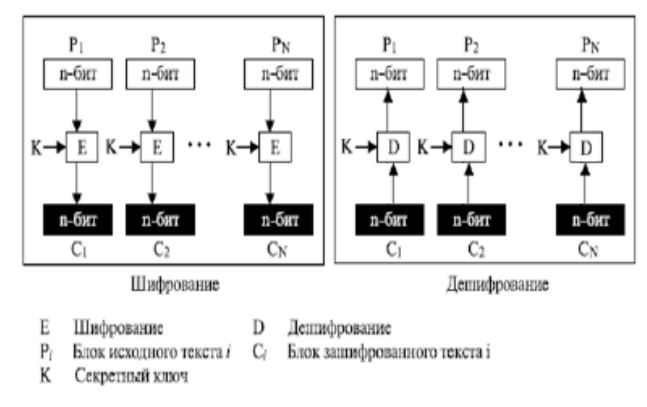
\includegraphics[width=\textwidth]{./img/S005.jpg}
        \caption{Режим ECB}%
        \label{img:1:5}
    \end{subfigure}%
    \hspace{2cm}
    \begin{subfigure}[b]{0.43\textwidth}
        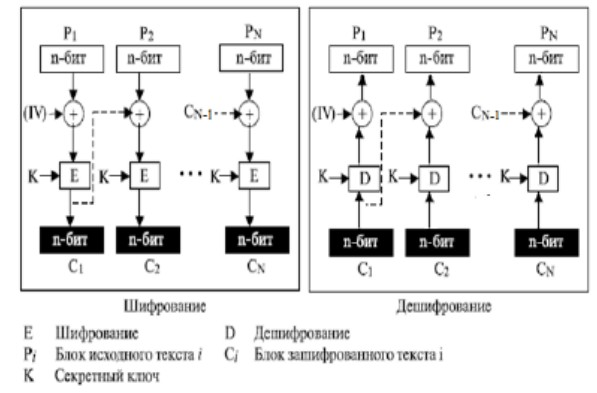
\includegraphics[width=\textwidth]{./img/S006.jpg}
        \caption{Режим CBC}%
        \label{img:1:6}
    \end{subfigure}
    \caption{Режимы DES}
\end{figure}


\subsection{Формулировка задания}
\begin{itemize}
    \item Создать картинку со своими ФИО (формат bmp).
    \item Зашифровать картинку шифром DES в режиме ECB.\@
    \item Зашифровать картинку шифром DES в режиме CBC c тем же ключом.
    \item Сохранить скриншоты картинок для отчета.
    \item Сжать исходную и 2 зашифрованных картинки средствами CrypTool. Зафиксировать размеры полученных файлов в таблице.
    \item Выбрать случайный текст на английском языке (не менее 1000 знаков) и зашифровать его DES в режиме ECB.\@
    \item Для одного и того же шифротекста оцените время проведения атаки «грубой силы» в случаях, когда известно n-4, n-6, n-8,.., 2 байт секретного ключа. Зафиксировать результаты измерений в таблице.
\end{itemize}

\subsection{Ход работы}
\begin{itemize}
    \item Создана картинка с ФИО автора в формате .bmp %chktex 26
    \begin{figure}[h]
        \centering
        
\includegraphics[width=0.7\textwidth]{./img/fio.jpg}
        \caption{ФИО автора}%
        \label{img:2:1}
    \end{figure}
    \begin{figure}[h]
        \centering
        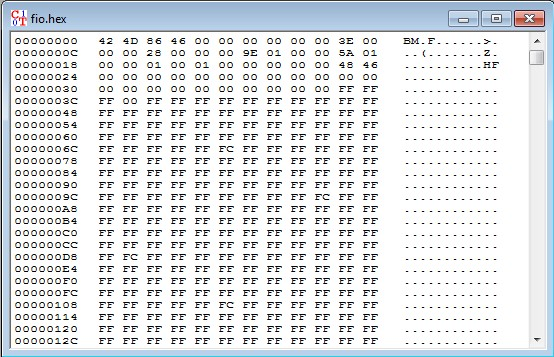
\includegraphics[width=0.7\textwidth]{./img/S009.jpg}
        \caption{fio.hex}%
        \label{img:2:2}
    \end{figure}
    \FloatBarrier{}
    \item В формате BMP первые 54 бита являются заголовком; их нужно убрать, чтобы потом можно было открыть расшифрованную картинку.\\
    Картинка зашифрована в режиме ECB ключом \texttt{88 00 55 53 53 50 63 04}. 54 бита из заголовка восстановлены. Результаты на рис.~\ref{img:2:3}.
    \begin{figure}[h]
        \centering
        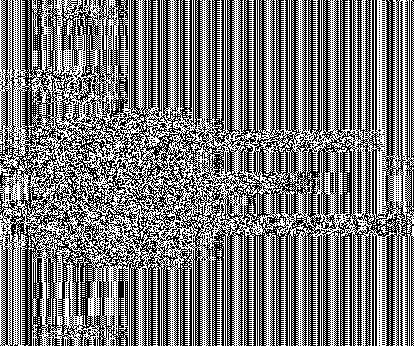
\includegraphics{./img/fio1.jpg}
        \caption{Шифрование DES (ECB)}%
        \label{img:2:3}
    \end{figure}
    Как можно видеть, из-за того, что блоки независимы, однаковые блоки шифруются одинаково. Контуры фигуры всё ещё видно.

    Если сделать изображение 16-битное, то становится видно ещё лучше (рис.~\ref{img:2:4})
    \begin{figure}[h]
        \centering
        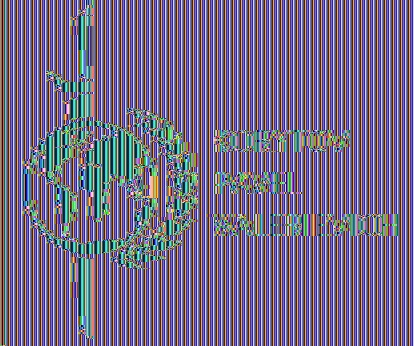
\includegraphics{./img/fio_16_1.jpg}
        \caption{Шифрование DES (ECB) для 16-битного изображения}%
        \label{img:2:4}
    \end{figure}
    \FloatBarrier{}
    \item Проведено шифрование в режиме CBC.\@ Изображение более неразличимо (рис.~\ref{img:2:5})
    \begin{figure}[h]
        \centering
        
\includegraphics{./img/fio2.jpg}
        \caption{Шифрование DES (CBC)}%
        \label{img:2:5}
    \end{figure}
    \item Произведено сжатие (Indiv. Procedures > Tools > Compression > Zip) получившихся файлов.
    \begin{table}[h]
    \centering
    \begin{tabular}{@{}ll@{}}
    \toprule
    \textbf{Файл} & \textbf{Процент сжатия} \\ \midrule
    \textit{Исходный} & $87\%$ \\
    \textit{DES (ECB)} & $66\%$ \\
    \textit{DES (CBC)} & $0\%$ \\ \bottomrule
    \end{tabular}
    \end{table}

    Как можно заметить, файл, сжатый DES в режиме CBC, не сжался вовсе

    \item Для шифрования взят абзац из книги Ричарда Докинза ``Delusion God''. Произведено зашифрование DES (ECB).
    \begin{figure}[h]
        \centering
        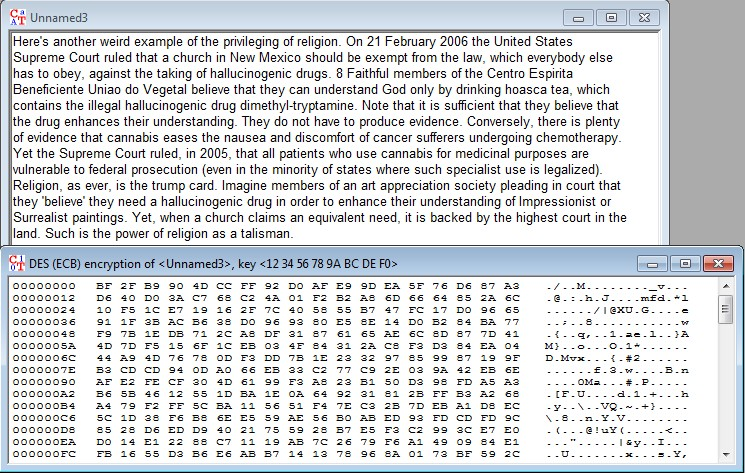
\includegraphics[width=\textwidth]{./img/S010.jpg}
        \caption{Шифрование }%
        \label{img:2:6}
    \end{figure}
    \item Исследовано время атак грубой силой на шифр, если известно некоторое количество байт ключа:
    \begin{table}[h]
        \centering
        \begin{tabular}{@{}llllll@{}}
        \toprule
        \textbf{Известно  байт} & 6 & 5 & 4 & 3 & 2 \\ \midrule
        \textbf{Время дешифровки} & 0 с & 21 с & 43 мин & 3.8 дней & 1.8 лет \\ \bottomrule
        \end{tabular}
    \end{table}

\end{itemize}

\FloatBarrier{}
\section{Исследование 3-DES}
\subsection{Описание}
Шифр 3-DES состоит в трехкратном применении обычного шифра DES.\@ Существуют 4 основные версии этого шифра:
\begin{enumerate}
    \item \texttt{DES-EEE3} --- шифрование происходит 3 раза независимыми ключасми
    \item \texttt{DES-EDE3} --- операция шифровка-расшифровка-шифровка с тремя разными ключами
    \item \texttt{DES-EEE2} --- то же, что и \texttt{DES-EE3}, но на первом и последнем шаге одинаковый ключ
    \item \texttt{DES-EDE2} --- то же, что и \texttt{DES-EDE2}, но на первом и последнем шаге одинаковый ключ\\
\end{enumerate}
На текущий момент самыми популярными разновидностями шифра являются \texttt{DES-EDE3} и \texttt{DES-EDE2}.

\subsection{Формулировка задания}
\begin{itemize}
    \item Выбрать случайный текст на английском языке (не менее 1000 знаков).
    \item Создать бинарный файл с этим текстом, зашифровав и расшифровав его DES на 0-м ключе.
    \item Снять и сохранить частотную и автокорреляционную характеристику этого файла.
    \item Зашифровать бинарный файл шифром 3-DES в режиме ECB.\@
    \item Снять и сохранить частотную и автокорреляционную характеристику файла с шифровкой.
    \item Зашифровать исходный бинарный файл 3-DES в режиме CBC c тем же ключом.
    \item Снять и сохранить частотную и автокорреляционнуюх арактеристику файла с шифровкой.
    \item Определить экспериментальным путем по какой схеме работает
        реализация 3-DES в CrypTool. Сохранить подтверждающие скриншоты.
\end{itemize}


\subsection{Ход работы}
\begin{enumerate}
    \item Выбран тот же текст, что и в предыдущем пункте
    \item Создан бинарный файл с текстом
    \begin{figure}[h]
        \centering
        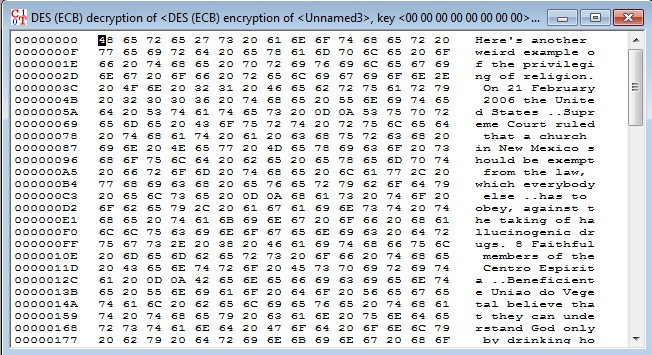
\includegraphics[width=0.7\textwidth]{./img/S011.jpg}
        \caption{Текст в бинарном виде}%
        \label{img:3:1}
    \end{figure}
    \item Снята частотная (рис.~\ref{img:3:2}) характеристика и автокорелляционная (рис.~\ref{img:3:3}) характеристика.
    \begin{figure}[h]
        \centering
        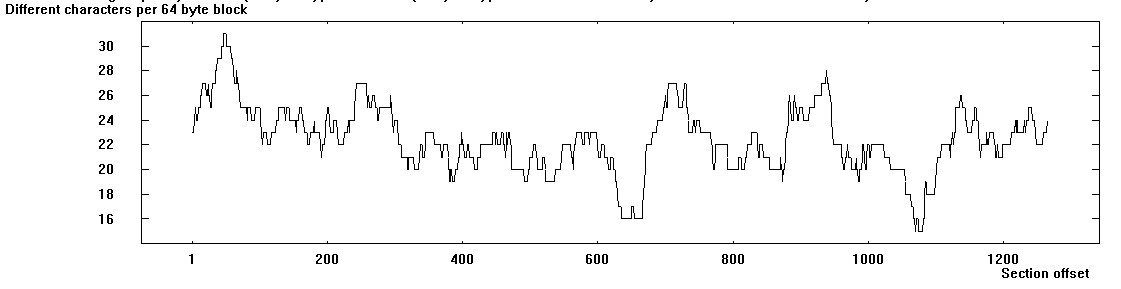
\includegraphics[width=\textwidth]{./img/S012.jpg}
        \caption{Частотная характеристика исходного текста}%
        \label{img:3:2}
    \end{figure}
    \begin{figure}[h]
        \centering
        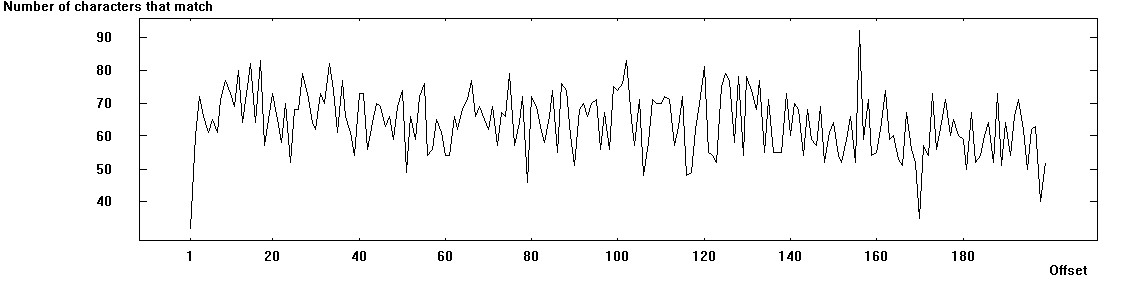
\includegraphics[width=\textwidth]{./img/S013.jpg}
        \caption{Автокорелляционная характеристика исходного текста}%
        \label{img:3:3}
    \end{figure}
    \FloatBarrier{}
    \item Произведено зашифрование 3-DES (ECB)
    \item Сняты те же характеристики для шифротекста (рис.~\ref{img:3:4},~\ref{img:3:5})
    \begin{figure}[h]
        \centering
        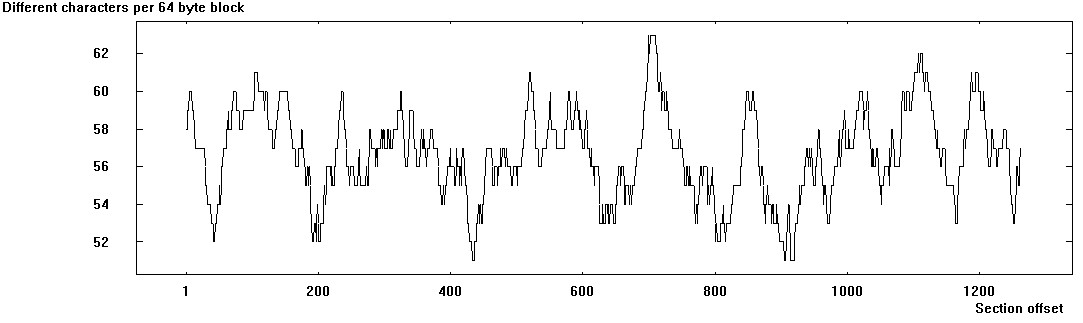
\includegraphics[width=\textwidth]{./img/S014.jpg}
        \caption{Частотная характеристика шифротекста 3-DES (ECB)}%
        \label{img:3:4}
    \end{figure}
    \begin{figure}[h]
        \centering
        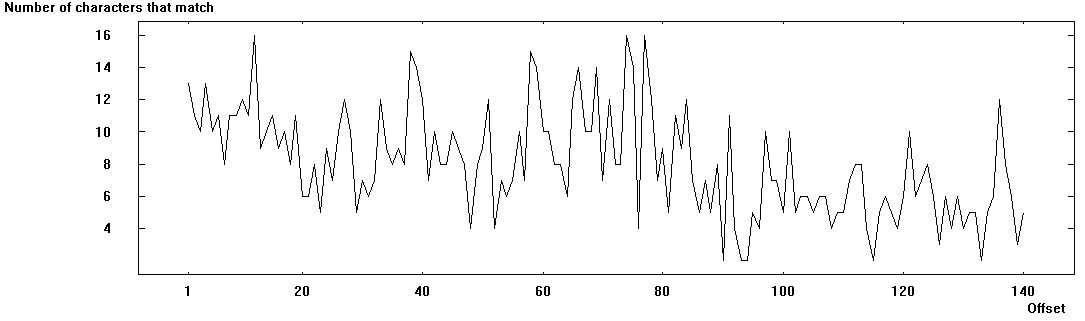
\includegraphics[width=\textwidth]{./img/S015.jpg}
        \caption{Автокорелляционная характеристика шифротекста 3-DES (ECB)}%
        \label{img:3:5}
    \end{figure}
    \item Произведено зашифрование 3-DES (CBC)
    \item Снова сняты частотная и автокорелляционная характеристики (рис.~\ref{img:3:6},~\ref{img:3:7})
    \begin{figure}[h]
        \centering
        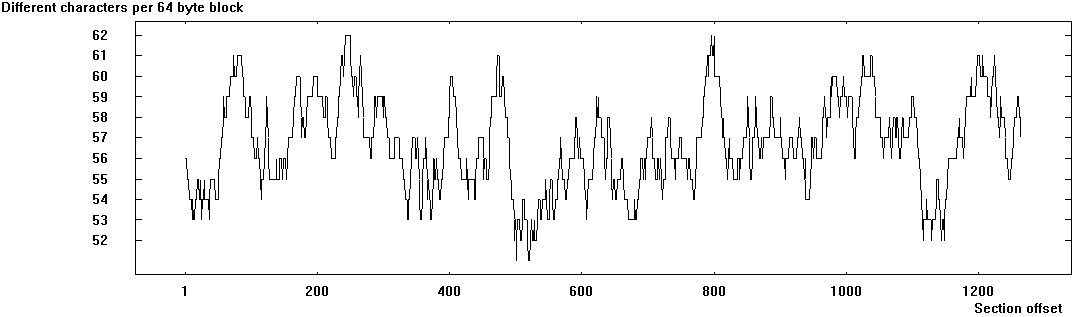
\includegraphics[width=\textwidth]{./img/S016.jpg}
        \caption{Частотная характеристика шифротекста 3-DES (CBC)}%
        \label{img:3:6}
    \end{figure}
    \begin{figure}[h]
        \centering
        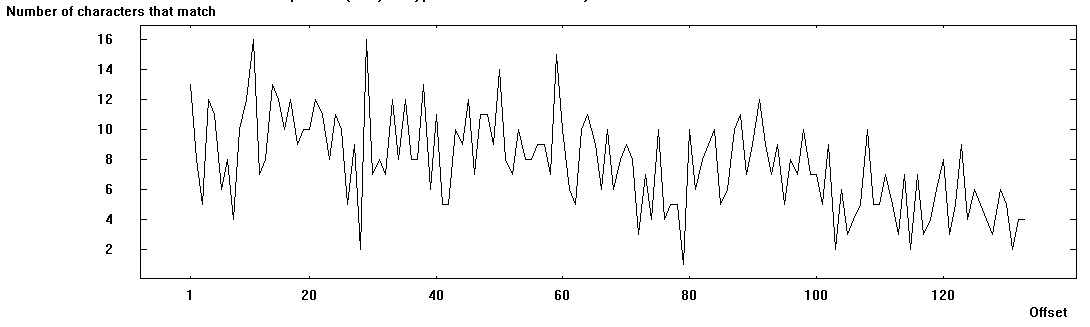
\includegraphics[width=\textwidth]{./img/S017.jpg}
        \caption{Автокорелляционная характеристика шифротекста 3-DES (CBC)}%
        \label{img:3:7}
    \end{figure}
    \item Используемая длина ключа --- 112 бит (рис.~\ref{img:3:8}), значит исключаются варианты DES-EEE3 и DES-EDE3.
    \begin{figure}[h]
        \centering
        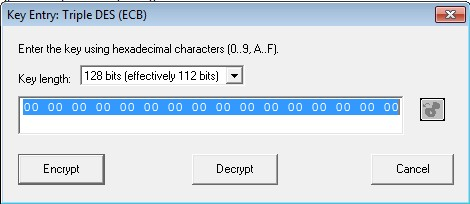
\includegraphics[width=0.7\textwidth]{./img/S018.jpg}
        \caption{Параметры шифра 3-DES}%
        \label{img:3:8}
    \end{figure}
    Чтобы выбрать между DES-EEE2 и DES-EDE2, произведено зашифрование текста нулевым ключом обычным DES и исследуемым 3-DES.\@ Результаты совпали (рис.~\ref{img:3:9}).
    \begin{figure}[h]
        \centering
        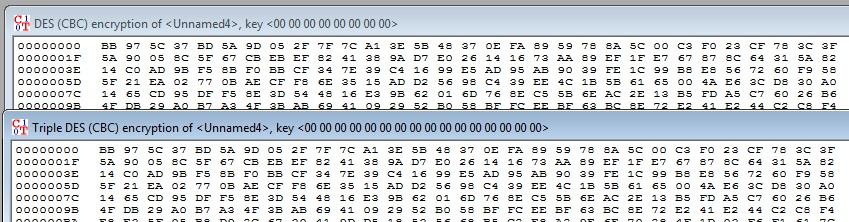
\includegraphics[width=\textwidth]{./img/S019.jpg}
        \caption{Шифрование 3-DES и DES}%
        \label{img:3:9}
    \end{figure}
    
    Совпадение результатов возможно, только если используется DES-EDE2 --- в таком случае расшифровка на втором этапе компенсирует зашифровку на 1-м.
\end{enumerate}

\section{Исследование модификаций DESX, DESL, DESXL шифра DES}
\subsection{Описание}
Алгоритм DESX используется на входе ключ длиной 184 бита, который делится на 3 56-битные части. Процесс шифрования происходит по следующей схеме:
\[ DESX(M) = K_2 \oplus DES_K (M \oplus K_1) \]
Если $K_1 = K_2 = 0$, то это обычный DES.\@

DESL отказывается от входной и выходной перестановки блока. 8 S-блоков заменяются на один, но более криптостойкий.

DESXL используется оптимизации DESL и производит шифрование по DESX.\@

\subsection{Формулировка задания}
\begin{itemize}
    \item Выбрать случайный текст на английском языке (не менее 1000 знаков).
    \item Создать бинарный файл с этим текстом, зашифровав и расшифровав его DES на 0-м ключе.
    \item С помощью CrypTool зашифровать текст с использованием шифров DESX, DESL, DESXL.\@
    \item Средствами CrypTool вычислить энтропию исходного текста и шифротекстов, полученных в итоге. Зафиксировать результаты измерений в таблице.
    \item Средствами CrypTool оцените время проведения атаки «грубой силы» при полном отсутствии информации о секретном ключе
\end{itemize}

\subsection{Ход работы}
\begin{enumerate}
    \item Выбран тот же текст, что и в предыдущем пункте.
    \item Описанным образом получен бинарный файл
    \item Произведено зашифрование текста с помощью DESX, DESL, DESXL (рисунок~\ref{img:4:1})
    \begin{figure}[h]
        \centering
        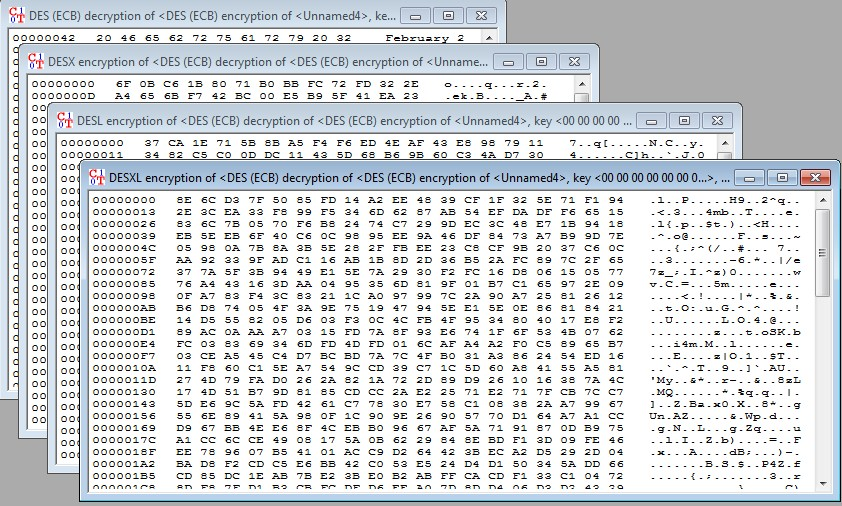
\includegraphics[width=0.7\textwidth]{./img/S020.jpg}
        \caption{Шифрование DESX, DESL, DESXL}%
        \label{img:4:1}
    \end{figure}
    \FloatBarrier{}
    \item Определена энтропия исходного текста и шифротекстов:
    \begin{table}[h]
    \centering
    \begin{tabular}{@{}ll@{}}
    \toprule
    \textbf{Текст} & \textbf{Энтропия} \\ \midrule
    \textit{Исходный} & 4.46 \\
    \textit{DESX} & 7.85 \\
    \textit{DESL} & 7.85 \\
    \textit{DESXL} & 7.83 \\ \bottomrule
    \end{tabular}
    \end{table}
    \item Произведена оценка времени атаки грубой силы на все шифротексты:
    \begin{table}[h]
    \centering
    \begin{tabular}{@{}ll@{}}
    \toprule
    \textbf{Шифр} & \textbf{Время атаки грубой силы (лет)} \\ \midrule
    \textit{DESX} & $4.8 \sbullet 10^{42}$ \\
    \textit{DESL} & $1.1 \sbullet 10^4$ \\
    \textit{DESXL} & $3.9 \sbullet 10^{42}$ \\ \bottomrule
    \end{tabular}
    \end{table}
\end{enumerate}

\newpage
\section*{Выводы}
\begin{table}[h]
    \centering
    \begin{tabular}{@{}llll@{}}
    \toprule
    \textbf{Шифр} & \textbf{Длина ключа (бит)} & \textbf{Brute force (лет)} & \textbf{Энтропия} \\ \midrule
    \textit{DES (EBC)} & 56 & $2 \sbullet 10^4$ & $7.85$ \\
    \textit{DES (CBC)} & 56 & $3.2 \sbullet 10^4$ & $7.84$ \\
    \textit{DES-EDE2 (EBC)} & 112 & $2.6 \sbullet 10^{21}$ & $7.84$ \\
    \textit{DES-EDE2 (CBC)} & 112 & $3 \sbullet 10^{21}$ & $7.85$ \\
    \textit{DESX} & 184 & $4.8 \sbullet 10^{42}$ & $7.85$ \\
    \textit{DESL} & 64 & $1.1 \sbullet 10^4$ & $7.85$ \\
    \textit{DESXL} & 184 & $3.9 \sbullet 10^{42}$ & $7.83$ \\ \bottomrule
    \end{tabular}
\end{table}
Исследованы разновидности блочного шифра DES.\@ Во всех случая размер блока --- 64 бит. Эффективный размер ключа меньше реального из-за битов четности.

Использование шифров в режиме EBC (все блоки независимы) для осмысленной информации (с низкой энтропией) значительно снижает криптостойкость, т.к. одинаковые блоки шифруются одинаково. Режим CBC лишен этого недостатка, но в этом случае невозможно распараллелить зашифрование.

Малая длина ключа --- другая проблема оригинального DES.\@ С использованием современного вычислительного оборудования, перебрать $2^{56}$ вполне возможно.

Использование модификации 3-DES значительно повышает криптостойкость алгоритма; перебор $2^{112}$ вариантов --- гораздо более трудоемкая задача.

Использование DESX --- более простой с вычислительной точки зрения способ повысить криптостойкость алгоритма. С точки зрения атаки полного перебора, это даже более эффективно, чем рассмотренный DES-EDE2.

Модификация DESL практически не снижает криптойкость DES, а DESXL --- DESX.\@

Знание части ключа шифрования значительно облегчает дешифровку. Таким образом, если используются слабые ключи (вроде 0630417 из данной л/р), и если это известно криптоаналитику, дешифрование значительно ускорится.

\end{document}
